% Section 4: Studies and Results II (writer-grounded validity; necessary but not sufficient; event/role structure;
% consultant-revised requirements; frontier limits). Every number is a \jm... macro from make_macros.py (function s4(), plus
% earlier functions). No hand-typed numbers. Quoted examples are stored outputs chosen by a declared rule, printed with their rate.
% Labels provided: sec:s4, sec:waterfall, sec:whole-message, sec:event-role, sec:validity, sec:slp, sec:req-revisions, sec:frontier.
% Cross-references used from other sections: sec:default, sec:guard, sec:design, sec:req.
% CITE-NEEDED (not opened, not in refs.bib): CLAM / Clarify When Necessary (Zhang and Choi, NAACL Findings 2025); COMPA (CHI 2024);
%   semantic entropy (Kuhn et al.; Farquhar et al.); contextual calibration (Zhao et al. 2021).
\section{Studies and Results II: Writer-Grounded Validity and the Limits of Commitment Preservation}\label{sec:s4}

Section~\ref{sec:default} and Section~\ref{sec:guard} establish that a missing cue is the main source of silent reversals and that a supplied cue, or a guard that deletes an unlicensed addition, removes most of them.
Those results are measured against a critical commitment: the one dimension that a minimal pair contrasts, labelled by automatic judges and a blind arbiter.
This section asks whether that measurement tracks what the people who write and use the messages mean by a correct draft.
It reports the studies in turn and then a set of bounded negative results.
In the writer-intent study (writer-intent study) the \jmpOneEightWriters{} writers of the human-written pairs rated drafts generated from their own pairs.
A whole-message analysis of those ratings separates the reasons a draft is rejected.
A human check of the arbitrated labels (arbiter check) measures how well each automatic judge and the arbiter agree with people.
Speech-language pathologists (SLPs; \jmdesignSlp{} raters) supply clinical severity weights and an acceptability review.
Two paid design consultants who use AAC (\jmdesignConsultants{} consultants) revise the requirement list; we know nothing of their communication or access method beyond that they use AAC, and nothing they said is treated as data.
The section closes with the frontier results that mark where asking, model uncertainty and partner context stop helping.
The result that organises the section is that preserving the critical commitment is necessary and far from sufficient, and that the shortfall has a specific structure.

\subsection{Writer-intent study}\label{sec:waterfall}

\paragraph{Design.}
Each of the \jmpOneEightWriters{} writers rated \jmpOneEightPerWriter{} drafts generated from their own kept pairs, half from the keywords alone (\emph{bare}) and half from the keywords plus the chip for the critical dimension (\emph{chip}).
Drafts came from the \jmwmModels{} primary models under the base prompt, and the draw was seeded and fixed before rating (\jmpOneEightAcceptN{} drafts in all).
For each draft the writer said which of their own two sentences it expresses (their sentence A, their sentence B, something else, or unclear) and whether they would accept it as their message (yes, yes with a small edit, or no), with a free-text note.
Writers were adult non-author university classmates who consented and were paid; the study measures writer-intent agreement, not validation by AAC users.
The automatic judge labels only the critical dimension, whereas the writer judges the whole message.
In the bare channel the keywords do not say which sentence the writer meant, so no model could know; the bare match rate is a reference level, not a failure rate, and the cue effect below is the measured value of supplying the missing commitment, not a claim that the chip is sufficient.

\paragraph{Results.}
Table~\ref{tab:s4-p18} gives the ratings.
Writers said the draft expressed the sentence the pair was generated from in \jmpOneEightMatchAll{}\% of rated drafts (\jmpOneEightMatchAllK{} of \jmpOneEightMatchAllN{}; 95\% interval \jmpOneEightMatchAllLo{} to \jmpOneEightMatchAllHi{}), and in \jmpOneEightElse{}\% they said it expressed something else.
The chip raises the intended-version match from \jmpOneEightMatchBare{}\% to \jmpOneEightMatchChip{}\%, a gain of \jmpOneEightCueGain{} points (writer-cluster interval \jmpOneEightCueGainLo{} to \jmpOneEightCueGainHi{}).
Writers accepted \jmpOneEightAcceptYesK{} of \jmpOneEightAcceptN{} drafts as written, and the one accepted draft came from the bare channel; \jmpOneEightAcceptYesSmall{}\% were acceptable as written or with a small edit.
Writers' agreement with the automatic judge on the four-way label (A, B, other, unclear) was \jmpOneEightAgreeFour{}\% ($\kappa$ = \jmpOneEightKappa{}).

\begin{table}[t]
\centering\small
\caption{Writer ratings of drafts generated from their own pairs (writer-intent study). Match: the writer says the draft expresses the sentence it was generated from. Bare is a reference level because the keywords do not determine the side. Intervals are 95\% Wilson over drafts; the cue contrast uses writer clusters.}\label{tab:s4-p18}
\begin{tabular}{@{}lrrrr@{}}
\toprule
Channel & Drafts & Match (\%) & Accepted as written & As written or small edit (\%) \\
\midrule
Bare & \jmpOneEightYesBareN{} & \jmpOneEightMatchBare{} [\jmpOneEightMatchBareLo{}, \jmpOneEightMatchBareHi{}] & \jmpOneEightYesBareK{} of \jmpOneEightYesBareN{} & \jmpOneEightSmallBare{} \\
Chip & \jmpOneEightYesChipN{} & \jmpOneEightMatchChip{} [\jmpOneEightMatchChipLo{}, \jmpOneEightMatchChipHi{}] & \jmpOneEightYesChipK{} of \jmpOneEightYesChipN{} & \jmpOneEightSmallChip{} \\
All & \jmpOneEightAcceptN{} & \jmpOneEightMatchAll{} [\jmpOneEightMatchAllLo{}, \jmpOneEightMatchAllHi{}] & \jmpOneEightAcceptYesK{} of \jmpOneEightAcceptN{} & \jmpOneEightAcceptYesSmall{} \\
\bottomrule
\end{tabular}
\end{table}

\paragraph{Is the acceptance criterion too strict?}
Two criteria are used on purpose and both are reported. ``Intended version'' asks whether the draft is the sentence the writer wrote, and ``accepted as written'' asks whether the writer would send it unchanged; both are strict, and the writer's own sentence contained words absent from the keywords in \jmwmDroppedUnrecShare{}\% of rejections, so some rejection is built into keyword input. A graded reading is therefore the better summary of how far drafts are from usable: \jmpOneEightAcceptYesSmall{}\% of drafts (\jmpOneEightAcceptYesSmallK{} of \jmpOneEightAcceptN{}) were acceptable as written or with a small edit, against \jmpOneEightAcceptNo{}\% (\jmpOneEightAcceptNoK{}) that the writer would not accept. The claim that commitment preservation is necessary but not sufficient does not rest on the strict criterion: it holds under the graded one, because the share needing no or a small edit is far below the share of drafts that keep the critical commitment. We did not collect an edit-distance measure, and we have not tested how many edits writers could make with the interface they would use.

\paragraph{From a correct commitment to an accepted draft.}
Table~\ref{tab:s4-waterfall} follows the drafts through three filters.
The judge marked the critical commitment correct in \jmwmRightN{} of \jmwmAllN{} drafts (\jmwmRightShare{}\%).
Among those, writers said the draft was the version they meant in \jmwmRightIntendedK{} of \jmwmRightIntendedN{} cases with an answer (\jmwmRightIntShare{}\%), and accepted \jmwmRightAccK{} as written.
The other direction is clean: where the judge marked the critical commitment wrong, the writer said the draft was not the intended version in \jmwmWrongNotIntK{} of \jmwmWrongNotIntN{} cases.
The automatic judge's failures are therefore real failures to the people who wrote the messages, and its passes are not sufficient.

\begin{table}[t]
\centering\small
\caption{From a correct critical commitment to an accepted draft (writer-intent study). Denominators are stated in each cell because some writer answers are unknown.}\label{tab:s4-waterfall}
\begin{tabular}{@{}lrrr@{}}
\toprule
 & All & Chip & Bare \\
\midrule
Drafts rated & \jmwmAllN{} & \jmpOneEightYesChipN{} & \jmpOneEightYesBareN{} \\
Judge: critical commitment correct & \jmwmRightN{} & \jmwmRightChipN{} & \jmwmRightBareN{} \\
\ \ and writer: it is the intended version & \jmwmRightIntendedK{} of \jmwmRightIntendedN{} & \jmwmRightChipIntK{} of \jmwmRightChipIntN{} & \jmwmRightBareIntK{} of \jmwmRightBareIntN{} \\
\ \ and writer: accepted as written & \jmwmRightAccK{} of \jmwmRightN{} & \jmwmRightChipAccK{} of \jmwmRightChipN{} & \jmwmRightBareAccK{} of \jmwmRightBareN{} \\
\bottomrule
\end{tabular}
\end{table}


\begin{figure}[t]
\centering
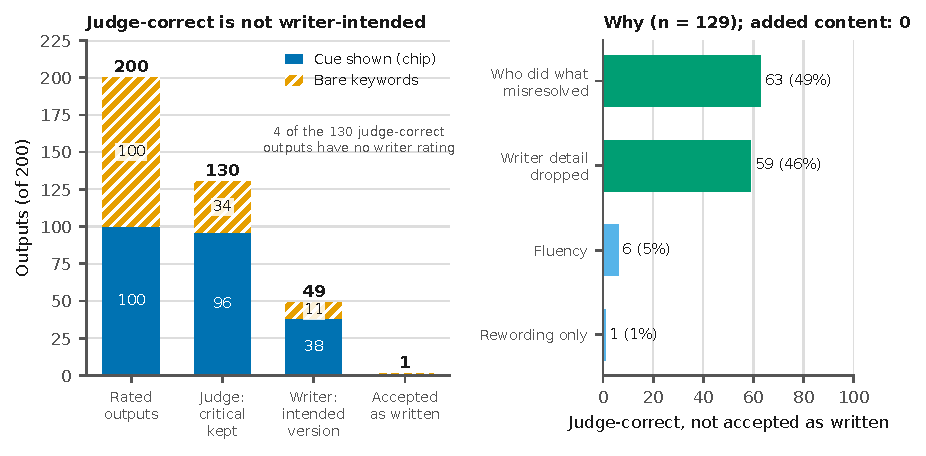
\includegraphics[width=\linewidth]{figs/fig2_waterfall.pdf}
\caption{Judge-correct is not writer-intended. Left: of \jmpOneEightAcceptN{} writer-rated outputs, \jmwmRightN{} keep the critical commitment by the judge, \jmwmRightIntendedK{} of the \jmwmRightIntendedN{} with a writer rating are the writer's intended version, and \jmpOneEightAcceptYesK{} is accepted as written. Right: reasons among the judge-correct outputs not accepted as written (writer-coded classification, kappa \jmwmHandKappa{} on a 40-item hand check); no output was coded as adding content.}\label{fig:waterfall}
\Description{Judge-correct is not writer-intended.}
\end{figure}

\subsection{Why correct drafts are rejected: the whole-message analysis}\label{sec:whole-message}

\paragraph{Method.}
For each of the \jmwmAllNotAccN{} drafts that writers did not accept as written, we assigned a primary reason from the writer's note and a lexical diff between the draft and the writer's own sentence: the critical commitment is wrong, a different event or role is expressed (substitution), writer detail is missing (dropped), content is added, the draft is not fluent, or it only rewords.
The analysis is post hoc and used no new model calls.
The diff classifier agrees with a hand coding of \jmwmHandN{} drafts in \jmwmHandAgree{}\% of cases ($\kappa$ = \jmwmHandKappa{}); the hand coder was an LLM and the classifier rules were written after seeing those drafts, so the agreement is an optimistic bound rather than a held-out estimate.
A second flag marks whether a content word of the writer's sentence is neither among the keywords nor a chip realisation, so that the model could not have known it.

\paragraph{Reasons.}
Table~\ref{tab:s4-reasons} gives the primary reasons by channel.
Without the cue, \jmwmBareCritical{}\% of non-accepted drafts fail on the critical commitment itself; with the chip that share falls to \jmwmChipCritical{}\%.
The cue converts violations into the two failures that remain: substitution (\jmwmChipSubst{}\%) and dropped writer detail (\jmwmChipDropped{}\%) among chip drafts.
Restricting to drafts whose critical commitment the judge marked correct and the writer did not accept as written (\jmwmRightNotAccN{} drafts), the primary reason is substitution in \jmwmRightSubst{}\% and dropped detail in \jmwmRightDropped{}\%; fluency accounts for \jmwmRightFluency{}\%.
Among the \jmwmROneN{} judge-correct drafts that writers said were not the intended version, \jmwmROneSubstK{} (\jmwmROneSubst{}\%) are substitutions and \jmwmROneDroppedK{} (\jmwmROneDropped{}\%) are dropped detail.

\begin{table}[t]
\centering\small
\caption{Primary reason a draft was not accepted as written (writer-intent study; share of non-accepted drafts; classifier validated against a hand coding, agreement \jmwmHandAgree{}\%). Fluency and rewording account for the remainder.}\label{tab:s4-reasons}
\begin{tabular}{@{}lrrr@{}}
\toprule
Primary reason & Bare (n=\jmwmBareNotAccN{}) & Chip (n=\jmwmChipNotAccN{}) & All (n=\jmwmAllNotAccN{}) \\
\midrule
Critical commitment wrong & \jmwmBareCritical{} & \jmwmChipCritical{} & \jmwmAllCritical{} \\
Event or role substituted & \jmwmBareSubst{} & \jmwmChipSubst{} & \jmwmAllSubst{} \\
Writer detail dropped & \jmwmBareDropped{} & \jmwmChipDropped{} & \jmwmAllDropped{} \\
Content added & --- & --- & \jmwmAdded{} \\
\bottomrule
\end{tabular}
\end{table}

\paragraph{Compression loss.}
In \jmwmRightUnrec{}\% of the judge-correct, non-accepted drafts the writer's sentence contains at least one content word that is neither a keyword nor a chip realisation.
The writers typed keywords because typing is slow; the details they meant (a place, a time, an object) were not in the input.
A draft is therefore a plausible completion of a compressed message and not a reconstruction of it, and the shortfall is a property of the task before it is a property of any model.
The appropriate response is a draft the writer can inspect, choose among and edit, which is the design the consultants asked for (Section~\ref{sec:req-revisions}).

\paragraph{Added content.}
Added content is never the primary reason for rejection in the writer data (\jmwmAdded{}\% of primary reasons).
As a secondary flag, \jmwmRightAddedFlag{}\% of judge-correct, non-accepted drafts contain a content word absent from the input.
We therefore do not claim that these drafts add unrequested content as the reason writers reject them.
The SLP panel applies a different standard, whether a sentence is safe to speak as a client's message with no writer sentence available, and there added content is prominent (Section~\ref{sec:slp}).

\paragraph{A deployable signal.}
Among judge-correct drafts, the ratio of draft length to the number of keywords given ranks the drafts that writers reject with AUROC \jmwmLenAuc{} (item-bootstrap interval \jmwmLenAucLo{} to \jmwmLenAucHi{}).
The critical label alone ranks writer rejection over all drafts at AUROC \jmwmCritAuc{}; the label plus three deployable features (judge added-content flag, length ratio, novel content words) reaches \jmwmCritPlusAuc{} (\jmwmCritPlusAucLo{} to \jmwmCritPlusAucHi{}) under cross-validation.
This is an observational association in \jmwmAllN{} drafts from \jmpOneEightWriters{} writers and identifies the drafts that say much more than the keywords gave; it is not a validated quality metric.

\paragraph{Examples.}
Table~\ref{tab:s4-examples} shows stored outputs chosen by a declared rule: among judge-correct drafts that writers said were not the intended version, for each primary reason the draft with the smallest SHA-256 of a fixed string and the item identifier.
The first two rows are writer-grounded; the last two are from the SLP panel, drawn by the same rule among judge-passed outputs that an SLP marked partly or no.

\begin{table*}[t]
\centering\small
\caption{Real stored outputs by declared rule. Rates: substitution \jmwmROneSubstK{} of \jmwmROneN{} and dropped \jmwmROneDroppedK{} of \jmwmROneN{} judge-correct drafts the writer said were not the intended version; SLP substitution \jmwmSlpSubstK{} and added \jmwmSlpAddedK{} of \jmwmSlpReasonN{} judge-passed rater-items marked partly or no.}\label{tab:s4-examples}
\begin{tabular}{@{}p{0.09\linewidth}p{0.17\linewidth}p{0.24\linewidth}p{0.2\linewidth}p{0.22\linewidth}@{}}
\toprule
Reason & Input & Writer's sentence or judgement & Draft & Note \\
\midrule
Substitution & \texttt{[SURE] taxi wait} & ``The taxi waits outside the main gate.'' & ``I am sure I need to wait for the taxi.'' & ``I wait for the taxi rather than the taxi waiting at the gate.'' \\
Dropped & \texttt{[SURE] soup warm} & ``The soup is warm in the kitchen.'' & ``The soup is definitely warm.'' & ``Adds definite certainty and omits the kitchen.'' \\
SLP: substitution & \texttt{[TELL] bus stop hospital} & SLP: says what was selected, no; acceptable, no & ``I need to go to the hospital from the bus stop.'' & ``Invents the speaker needing hospital travel instead of stating something about the bus stopping at the hospital.'' \\
SLP: added & \texttt{please put soup bowl} & SLP: partly; acceptable with edit & ``Please put the soup bowl on the table.'' & ``Remove the invented table; confirm soup into a bowl versus moving a soup bowl.'' \\
\bottomrule
\end{tabular}
\end{table*}

\subsection{Event and role structure as a commitment dimension}\label{sec:event-role}

The commitment vector used so far has \jmdesignDims{} dimensions.
The whole-message analysis shows a failure that none of them names: the draft says something that is fluent, keeps the negation, the speech act and the tone, and nevertheless assigns the wrong participants to the wrong event.
``I am sure I need to wait for the taxi'' keeps the certainty chip and changes who does what.
We propose event and role structure as an additional commitment dimension, defined as the event the message describes and the participants that fill its roles (who acts, who or what is acted on, where or for whom), including the event to which a negation or modal attaches.
It differs from the existing agent dimension in scope: agent covers who performs the stated action, whereas event and role structure covers whether the action, its participants and its negation scope are the ones the writer meant.
Because the judge labels only the dimension a pair contrasts, a role error on an item whose contrast is certainty is not counted.

Three independent sources point to the same dimension.
First, substitution is the leading primary reason among judge-correct rejections (\jmwmRightSubst{}\%) and the leading reason among drafts the writer said were not the intended version (\jmwmROneSubst{}\%).
Second, in the SLP panel substitution is a primary reason for \jmwmSlpSubstK{} of \jmwmSlpReasonN{} outputs the judge passed and the SLP marked partly or no.
Third, the design consultants asked for relations to be preserved without being shown this analysis: one asked that the negation attach to the intended action, the other that the system preserve ``who reads, what is negated, and what the sentence is about'' (Section~\ref{sec:req-revisions}).
Both also rejected drafts in which a button such as TELL became a spoken verb that created a new event of telling someone.
We state the dimension as a proposal.
It has no detector and no human-validated rate in this paper, and the substitution label comes from a rule-based diff classifier (agreement with hand coding \jmwmHandAgree{}\%), not from a role-level annotation.

\subsection{Judges, arbiter and experts against people}\label{sec:validity}

\paragraph{Human check of arbitrated labels (arbiter check).}
The \jmpOneNineUnits{} units on which the two automatic judges disagreed were labelled by a blind, output-text-only arbiter.
Each unit was coded again by two of \jmpOneNineAnnotators{} adult annotators (classmates, consented, paid); unsure and missing answers were excluded, leaving \jmpOneNineCodings{} codings on the arbiter units.
People agree with the arbiter on \jmpOneNineAgreeArb{}\% of codings (interval \jmpOneNineAgreeArbLo{} to \jmpOneNineAgreeArbHi{}; $\kappa$ = \jmpOneNineKappaArb{}), against \jmpOneNineAgreeJOne{}\% for judge~1 ($\kappa$ = \jmpOneNineKappaJOne{}) and \jmpOneNineAgreeJTwo{}\% for judge~2 ($\kappa$ = \jmpOneNineKappaJTwo{}).
Where both coders gave the same label, the arbiter matches it for \jmpOneNineItemAgreeArbK{} of \jmpOneNineItemAgreeArbN{} units (\jmpOneNineItemAgreeArb{}\%), and the two coders agree with each other on \jmpOneNineHumanHumanArb{}\% of units.
The arbiter sided with judge~1 on \jmpOneNineSidedJOne{}, with judge~2 on \jmpOneNineSidedJTwo{} and with neither on \jmpOneNineSidedNeither{} units.
The units are the hardest by construction, so these rates compare the judges with each other and with people on disputed outputs; they are not overall judge accuracy.
They support using the arbiter label, without a fallback to judge~1, in every primary estimate.

\paragraph{``Can you \dots?'' as a request.}
Stored outputs of the form ``Can you \dots?'' (\jmpOneNineCanYouItems{} items) were coded by the same annotators as a request or command by \jmpOneNineCanYouRequest{}\% of codings (\jmpOneNineCanYouK{} of \jmpOneNineCanYouN{}; interval \jmpOneNineCanYouRequestLo{} to \jmpOneNineCanYouRequestHi{}).
The alternative coding, as a yes/no question, is not what these readers do, and the primary codebook codes the form as a request.

\paragraph{Writers and SLPs against the judge.}
Writers agree with the judge on the four-way label for \jmpOneEightAgreeFour{}\% of drafts ($\kappa$ = \jmpOneEightKappa{}).
On the SLP panel the judge's meaning-pass agrees with an SLP's judgement that the output says what the selected words mean at $\kappa$ = \jmslpJudgeKappaOne{} and \jmslpJudgeKappaTwo{} for the two SLPs (\jmslpItemsRated{} outputs).
The pattern matches the writer data.
The SLPs marked \jmwmSlpFailK{} of the \jmwmSlpFailN{} rater-items the judge failed as partly or no, and \jmwmSlpPassPartlyK{} of the \jmwmSlpPassN{} the judge passed (\jmwmSlpPassPartly{}\%).
Excluding outputs on which the judge flagged added content, \jmwmSlpPassNoAddK{} of \jmwmSlpPassNoAddN{} (\jmwmSlpPassNoAdd{}\%) were still marked partly or no.
Neither human group disputes the judge's failures; neither confirms its passes.
The automatic judges are screening instruments whose failures are informative and whose passes need a human or arbiter check, which is the role they play in the primary estimates.

\subsection{Speech-language pathologist review}\label{sec:slp}

\paragraph{Design.}
We engaged \jmdesignSlp{} practising SLPs as expert annotators of study materials, anonymously and under a written professional-services agreement.
They collected no personal data and the ratings concern outputs, not the raters.
For each of \jmslpTypesN{} kinds of silent meaning change they rated, on an anchored five-point scale, how serious the change would be if spoken as a client's message, and whether a system should block or flag it.
They then rated \jmslpItemsRated{} stored outputs drawn by a seeded rule fixed before rating (guard repairs, the original outputs for the same inputs, and chip and plain-word-cue outputs for the same inputs, with arm labels hidden) on whether each says what the selected words mean and whether it is acceptable to speak as the client's message.
We weight each judge-flagged failure by the SLP severity of its type, take the largest weight among the types flagged on an output, and report the mean over outputs next to the unweighted rate.
The panel is an expert review of a fixed set of outputs and not a population estimate.

\paragraph{Severity.}
The SLPs rated a dropped or added negation as the most serious change (mean \jmslpNegSeverity{} of 5) and both would block it; the same two raters would flag every one of the \jmslpTypesN{} types (\jmslpFlagTypesK{} of \jmslpTypesN{}) but block only \jmslpBlockTypesK{}.
Politeness added or removed was the least serious type (mean \jmslpSevPolite{}) and certainty the next lowest (mean \jmslpSevCert{}); Table~\ref{tab:s4-sev} gives all types.

\begin{table}[t]
\centering\small
\caption{SLP severity by type of silent meaning change (mean of two raters; 1 trivial to 5 critical). The weight is the mean divided by 5.}\label{tab:s4-sev}
\begin{tabular}{@{}lr@{}}
\toprule
Type of change & Mean severity \\
\midrule
Negation dropped or added & \jmslpNegSeverity{} \\
Question, statement or command changed & \jmslpSevSent{} \\
Actor switched & \jmslpSevActor{} \\
Time changed & \jmslpSevTime{} \\
Added content & \jmslpSevAdded{} \\
Certainty added or removed & \jmslpSevCert{} \\
Politeness added or removed & \jmslpSevPolite{} \\
\bottomrule
\end{tabular}
\end{table}

\paragraph{Clinically weighted failure.}
Table~\ref{tab:s4-weighted} applies the weights to the judge-flagged failures in two populations; arms are compared only within a population.
On fresh speech-act families the guard lowers the weighted failure rate from \jmslpWGuardBase{}\% to \jmslpWGuardG{}\% (unweighted \jmslpUGuardBase{}\% to \jmslpUGuardG{}\%); the deletion-only variant reaches \jmslpWGuardGs{}\%.
On the human-written pairs the weighted failure rate is \jmslpWCueBare{}\% for bare keywords, \jmslpWCueChip{}\% with the chip and \jmslpWCueWord{}\% with the plain word.
A cue that carries no information about the critical dimension does not help: a non-critical cue gives \jmslpWCueNoncrit{}\% and an irrelevant chip \jmslpWCueIrrel{}\%.
Weighting compresses the unweighted rates without reordering the arms.

\begin{table}[t]
\centering\small
\caption{Failure rate (\%) unweighted and weighted by SLP severity. W-C: fresh speech-act families (\jmslpWcN{} targets); hw1: human-written pairs, six dimensions (\jmslpHwN{} targets). Weighted rate: the largest SLP weight among the types the judge flagged on an output, averaged over outputs.}\label{tab:s4-weighted}
\begin{tabular}{@{}llrr@{}}
\toprule
Population & Arm & Unweighted & Weighted \\
\midrule
W-C & Baseline & \jmslpUGuardBase{} & \jmslpWGuardBase{} \\
W-C & Guard & \jmslpUGuardG{} & \jmslpWGuardG{} \\
hw1 & Bare & \jmslpUCueBare{} & \jmslpWCueBare{} \\
hw1 & Chip & \jmslpUCueChip{} & \jmslpWCueChip{} \\
hw1 & Plain word & \jmslpUCueWord{} & \jmslpWCueWord{} \\
\bottomrule
\end{tabular}
\end{table}

\paragraph{Acceptability.}
The SLPs judged \jmslpAccRepair{}\% of guard repairs acceptable to speak as they stand (\jmslpAccRepairN{} rater-judgments), against \jmslpAccOrig{}\% of the original outputs for the same inputs (\jmslpAccOrigN{}); on the \jmslpPairN{} paired rater-judgments, \jmslpPairRepOnlyK{} were acceptable only after repair, \jmslpPairOrigOnlyK{} only before, and \jmslpPairBothK{} both.
With one small edit, \jmslpRepairEdit{}\% of repairs and \jmslpOrigEdit{}\% of originals were acceptable.
Chip outputs were acceptable as they stand in \jmslpAccChip{}\% of rater-judgments and plain-word outputs in \jmslpAccWord{}\% (\jmslpAccChipN{} each).
The two SLPs agree on whether an output says what the selected words mean at $\kappa$ = \jmslpKappaA{} and on acceptability at $\kappa$ = \jmslpKappaB{}.
These statistics describe these two raters on these outputs and have no sampling distribution over raters; intervals resample items only.
They are a different question from the classmate audit of Section~\ref{sec:guard} (``usable''), and the two should not be subtracted.

\subsection{Consultant-revised requirements}\label{sec:req-revisions}

\paragraph{Process.}
This was design consultation, not research participation. We engaged \jmdesignConsultants{} paid design consultants who use AAC (as they told us; we did not verify or ask about their access method or experience with keyword or language-model tools) to review the requirement list (R1 to R5) in plain language, with real example outputs and a description of the chip and plain-word designs, under a written consulting agreement.
They rated each requirement, said what was wrong or missing, named a rule we had forgotten and a list of things a system should never change without asking, indicated a preference between chips and plain words, and judged \jmconsExN{} example outputs as acceptable to send or not.
We collected no demographic, health or communication information and report neither their experiences nor any inference about AAC users in general: the consultants are not a sample, and their input is a set of changes to our proposed requirements, which remain proposals.

\paragraph{Result.}
In their written feedback both consultants rated the requirements R1 to R5 as important and neither asked for one to be dropped; we record this as a log of design feedback and not as a finding.
Table~\ref{tab:s4-changes} lists the suggestions that changed the list or our practice, with the source and the change adopted in this manuscript.
The central change is an additional requirement, R6: a generated sentence remains a draft until the person approves it, and drafting or editing never speaks or sends a message.
It reframes the evaluation question.
A silent reversal that is spoken is a communication failure; a wrong draft that is inspected costs reading and taps.
Approval cannot catch what the writer does not notice, so R6 does not replace the commitment filter, and it makes the coverage of the writer's whole intended message per draft read the quantity that matters.

% TODO-AUTHOR: the right-hand column states the dispositions adopted in this manuscript's requirement list (no closed feedback log with counts exists in the repo); confirm each before submission.
\begin{table*}[t]
\centering\small
\caption{Consultant suggestions (C1, C2) and the change adopted in the requirement list. Summaries paraphrase the stored written answers; none concerns a person's own communication.}\label{tab:s4-changes}
\begin{tabular}{@{}p{0.43\linewidth}p{0.07\linewidth}p{0.42\linewidth}@{}}
\toprule
Suggestion & From & Change to requirements or practice \\
\midrule
A draft is never spoken or sent without the person's action; provide a clear speak action, an editable preview and quick undo; keep the original words available to speak directly. & C1, C2 & New R6 (approval before speech); original words always speakable. \\
Complete typed sentences are kept exactly by default; rewriting only on explicit request, with the proposed change and the original shown, and undo. & C1, C2 & R2 restated as an exact-copy default with an optional, approval-gated rewrite. \\
Show a small number of meaningfully different drafts with the difference highlighted, or the one unresolved choice; do not chain questions; keep choices brief and reversible; do not learn a permanent preference from one answer. & C1, C2 & R3 restated: show differing drafts or the specific unresolved choice, not a questionnaire. \\
Preserve relations as well as button labels: the negation attaches to the intended action; a button such as TELL sets sentence form and must not become a verb or create an event of telling. & C1, C2 & R1 and R4 restated at the level of relations; event and role structure proposed as a commitment dimension (Section~\ref{sec:event-role}). \\
A never-change-without-asking list: yes or no, scope of not, who acts or receives, ownership, permission, names and places, amounts, event time, certainty, question versus statement versus command, explicit tone. & C1, C2 & Adopted as the protected scope; adds ownership, permission, names and places, and amounts to the dimensions measured in this paper. \\
The R2 bad example uses keywords and PLAIN and so does not show a typed sentence being changed; the chip and plain-word mockups differ in tense and time and cannot establish which is easier; a ``would be nice'' input was encoded as MAYBE. & C1, C2 & Treated as defects of the review materials, not of the requirements; R5 now requires equivalent content in both input styles. \\
Which is easier to imagine, a chip or a plain word: one chose the chip as a design preference, the other said it depends on access method; both asked that the actual selection effort be tested. & C1, C2 & No change: we make no claim about which input is easier, and tap cost is a proxy only. \\
\bottomrule
\end{tabular}
\end{table*}

\paragraph{Example outputs as a design illustration.}
We also showed the consultants \jmconsExN{} stored example outputs drawn by a hash-seeded rule (\jmconsGoodN{} the judge passed, \jmconsBadN{} it failed and \jmconsRepN{} guard repairs shown with the first try) and asked whether each was fine to send. We use their answers only as design feedback and report no tally of verdicts. Two of the judge-passed examples were set aside by both consultants because they invent a telling event that the selected buttons do not contain (``They will tell you about the club offer'' for \texttt{[YES] [TELL] [THEY] club offer}), which is the substitution pattern of Section~\ref{sec:event-role} appearing in a judge-passed output. A guard repair that removed ``please'' but kept the unselected state ``on'' (``Leave the light on'' from \texttt{[ASK] leave light}) was not accepted either, which shows that a deletion-only repair removes an unlicensed addition and leaves an uncued one. These cases informed the requirement changes above; \jmconsExN{} outputs do not support an estimate.

\subsection{Frontier limits: asking, model uncertainty and partner context}\label{sec:frontier}

The preceding results suggest several tempting ways to avoid supplying a cue on every message: ask the writer only when it matters, let the model's own uncertainty decide, or let the conversation partner's last remark supply context.
We tested each in a controlled, machine-labelled study.
All labels in this subsection are machine labels (two judges with a blind arbiter), the studies are pilot-scale and post-pilot rounds are marked as such in the evidence files, and no human has yet checked them.
% SLOT: human checks of the frontier labels enter here when scored.

\paragraph{Ask policies.}
The ask-policy comparison of Section~\ref{sec:asks} (Figure~\ref{fig:frontier}) is the first of these tests: no ranking rule, including a clarification-style trigger, beats asking at random among messages that lack the cue at matched taps, and supplying the cue on every message (\jmfOneRevPolChip{} polarity reversals per 1,000 with a chip, \jmfOneRevPolWord{} with a plain word) undercuts them.
A learned gate that uses model internals averts a modest share of SLP-weighted speech-act reversals under simulated resolution rates, but a supervised entropy-feature learner matches it; we treat that study as an evaluation framework and not as a result.

\paragraph{The model's own uncertainty does not flag the reversals.}
We asked whether default decoding hides a calibrated distribution over the dropped negation, using \jmknsModels{} local models, an untruncated sampler and \jmknsUnitsCap{} messages in which the negation was removed from every keyword string (a stress test) and a set of human keyword messages. % CITE-NEEDED: semantic entropy; contextual calibration
For Qwen2.5-7B, the model for which both datasets agree, sampled negation appears in \jmknsCapSampled{}\% of samples against a source rate of \jmknsCapTarget{}\% on the stress set, and in \jmknsHumSampled{}\% against \jmknsHumTarget{}\% on human keywords: the model is overconfident, not hiding a calibrated tail.
The sampled share ranks which inputs lost their negation at AUROC \jmknsAucKOneSixQwen{} and \jmknsAucKOneSixLlama{} for the two models, against \jmknsAucLex{} for a model-free classifier on the keywords alone.
A continuous score from the negation-token probability mass reaches \jmknsAucNegmass{} (\jmknsAucNegmassLo{} to \jmknsAucNegmassHi{}); its difference from the keyword classifier is $\jmknsNegmassVsLex$ [$\jmknsNegmassVsLexLo$, $\jmknsNegmassVsLexHi$], so a per-input signal exists but is no better than a model-free one.
A verbalised-probability score from one API model reaches \jmknsAucTerraVerbal{}, a difference of $\jmknsTerraVsLex$ [$\jmknsTerraVsLexLo$, $\jmknsTerraVsLexHi$] from the keyword classifier; its interval touches zero, so we treat it as a lead for a confirmatory run and not as a result.
The conclusion for design is that the model cannot be asked whether it dropped a cue more cheaply than the writer can be asked for the cue.

\paragraph{Partner context improves defaults and adds an echo.}
Giving the model the conversation partner's last remark is a published way to improve expansion accuracy~\cite{cai2022abbrev}, and we tested whether it also moves the polarity default.
With \jmpcFamilies{} polarity families, \jmpcModels{} models and model-written partner remarks, a negative remark raises the share of negated bare output by $\jmpcAll$ points [$\jmpcAllLo$, $\jmpcAllHi$], mostly by echoing the remark or agreeing with it.
Excluding verbatim echoes and agreement replies, the excess is $\jmpcProp$ points [$\jmpcPropLo$, $\jmpcPropHi$]; it depends on who wrote the remarks, from $\jmpcAuthQwen$ with one remark author to $\jmpcAuthMistral$ with the other on the \jmpcAuthFamilies{} families written by both.
A supplied polarity cue largely removes it: the excess is $\jmpcCue$ points [$\jmpcCueLo$, $\jmpcCueHi$] when echoes and agreements are counted as harm, and $\jmpcCueLow$ [$\jmpcCueLowLo$, $\jmpcCueLowHi$] when they are not.
A question remark does not raise the affirmative default; it lowers the affirmative share by $\jmpcQAff$ points through abstention.
The study is a controlled demonstration with templated remarks.
It says nothing about the rate in real AAC conversation or about whether echoing a remark the writer agrees with is harmful, and no zero-tap mitigation we tried beat random asking at matched taps.

\paragraph{What the limits establish.}
Taken together, these results fix the role of the cue.
Asking, model uncertainty and partner context each reduce reversals only partly or at a tap cost that a cue-on-every-message policy undercuts on the measured dimensions, and the cue still has to be elicited from the writer.
The remaining problem is not the trigger but covering the writer's whole intended message from a compressed input, which Sections~\ref{sec:waterfall} and~\ref{sec:req-revisions} show is a question about approval-gated drafts and not about a better filter.
